\chapter{QALU's Implementation with the Qiskit SDK}

In this chapter we will present five individual quantum circuits that perform fundamental arithmetic and logic
operations: addition, subtraction, multiplication and magnitude comparisons (less, greater than or equal). We
are also going to present the Python code that implement those circuits as well as their diagrammatic representations.

\section{The Quantum Half Adder}
In this section we are going to construct, using the Qiskit SDK, a quantum circuit that implements the classic Half-Adder circuit.
First we shall consider the classic circuit diagram of the Half-Adder circuit from Chapter 2.

\subsection{Analysing the diagram and logic of the Quantum Half-Adder}

\begin{figure}[!ht]
    \centering
    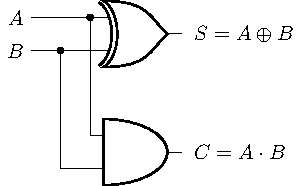
\includegraphics{images/5_Implementation/classical_halfadder_diagram.pdf}
    \caption{The classical Half-Adder circuit diagram}
\end{figure}

The circuit takes two 1-bit inputs, $A$ and $B$ and produces two 1-bit outputs $S$ (the sum, $A + B$) and $C$ (the possible carry of $S$).
As we can see from the diagram, to compute the sum of the inputs we have to apply an XOR gate on the inputs. As for the carry, we apply the
AND gate. From this simple analysis we can produce the truth table of this circuit to better construct its quantum-counterpart.

\begin{table}[!ht]
    \centering
    \begin{tabular}{c c|c c}
        $A$ & $B$ & $S = A \oplus B$ & $C = A \cdot B$ \\
        \hline
        $0$ & $0$ & $0$ & $0$ \\
        $0$ & $1$ & $1$ & $0$ \\
        $1$ & $0$ & $1$ & $0$ \\
        $1$ & $1$ & $0$ & $1$ \\
    \end{tabular}
    \caption{The truth table of the classical Half-Adder circuit}
\end{table}

Now the construction of the quantum Half-Adder is matter of matching the boolean functions, the XOR and AND function to be exact, to the
appropriate quantum gates.

Let $A$ and $B$ be two 1-qubit inputs. The XOR boolean function maps directly with the Feynman gate (or controlled-NOT/CNOT gate). We can deduce that
from comparing the two gates truth table.

\begin{table}[!ht]
    \centering
    \begin{subtable}[h]{0.45\textwidth}
        \centering
        \begin{tabular}{cc|c}
            $\ket{A}$ & $\ket{B}$ & $\ket{B}'=\ket{A \oplus B}$ \\
            \hline
            $0$ & $0$ & $0$ \\
            $0$ & $1$ & $1$ \\
            $1$ & $0$ & $1$ \\
            $1$ & $1$ & $0$ \\
        \end{tabular}
        \caption{CNOT's truth table}
    \end{subtable}
    \begin{subtable}[!h]{0.45\textwidth}
        \centering
        \begin{tabular}{cc|c}
            $A$ & $B$ & $A \oplus B$ \\
            \hline
            $0$ & $0$ & $0$ \\
            $0$ & $1$ & $1$ \\
            $1$ & $0$ & $1$ \\
            $1$ & $1$ & $0$ \\
        \end{tabular}
        \caption{XOR's truth table}
    \end{subtable}
    \caption{The truth tables of the CNOT (a) and XOR (b) gates side-by-side}
\end{table}

We omitted the third column from table (a) to better emphasize the similarities of the two gates.

The AND boolean function cannot be mapped directly to any quantum gate/operation because it is not reversible. This does not mean that it is
impossible to construct the same functionality using quantum gates. We shall borrow a \say{garbage} qubit $\ket{O} = 0$ to simulate the boolean AND function.
By applying the Toffoli gate with control qubits $\ket{A}$, $\ket{B}$ and the borrowed qubit $\ket{O}$, as the target, we simulate the AND functionality
directly.

\begin{figure}[!ht]
    \centering
    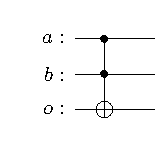
\includegraphics{images/5_Implementation/toffoli_gate_diagram.pdf}
    \caption{The Toffoli gate diagram}
\end{figure}

At the end of the computation, $\ket{O}$ will store the conjunction of $\ket{A}$ and $\ket{B}$. This can be seen more clearly from the side-by-side
view of the truth tables of the two gates.

\begin{table}[!ht]
    \centering
    \begin{subtable}[h]{0.45\textwidth}
        \centering
        \begin{tabular}{ccc|c}
            $\ket{A}$ & $\ket{B}$ & $\ket{O}$ & $\ket{O}'=\ket{A \cdot B}$ \\
            \hline
            $0$ & $0$ & $0$ & $0$ \\
            $0$ & $1$ & $0$ & $0$ \\
            $1$ & $0$ & $0$ & $0$ \\
            $1$ & $1$ & $0$ & $1$ \\
        \end{tabular}
        \caption{CCNOT's truth table}
    \end{subtable}
    \begin{subtable}[h]{0.45\textwidth}
        \centering
        \begin{tabular}{cc|c}
            $A$ & $B$ & $A \cdot B$ \\
            \hline
            $0$ & $0$ & $0$ \\
            $0$ & $1$ & $1$ \\
            $1$ & $0$ & $1$ \\
            $1$ & $1$ & $0$ \\
        \end{tabular}
        \caption{AND's truth table}
    \end{subtable}
    \caption{The truth tables of the Toffoli/CCNOT (a) and AND (b) gates side-by-side}
\end{table}

The complete circuit has to be constructed with caution because if we apply the CNOT gate first, we inevitably change the state of $\ket{B}$. With this
knowledge at hand we have to apply the CCNOT gate as the first computational step and later the CNOT gate.

\begin{figure}[!ht]
    \centering
    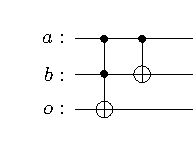
\includegraphics{images/5_Implementation/half_adder.pdf}
    \caption{The quantum Half-Adder circuit with slices that indicate each computational step}
\end{figure}

We are going to enumerate over each computational step:
\begin{enumerate}
    \item $\ket{O'} = CCNOT\ket{A}\otimes\ket{B}\otimes\ket{O} = CCNOT\ket{A,B,O} = \ket{A \oplus B}$
    \item $\ket{B'} = CNOT\ket{A}\otimes\ket{B} = \ket{A \cdot B}$
\end{enumerate}

\begin{table}[!ht]
    \centering
    \begin{tabular}{ccc|ccc}
        $\ket{A}$ & $\ket{B}$ & $\ket{O}$ & $\ket{A'} = \ket{A}$ & $\ket{B'} = \ket{C}$ & $\ket{O'} = \ket{S}$ \\
        \hline
        $0$ & $0$ & $0$ & $0$ & $0$ & $0$ \\
        $0$ & $1$ & $0$ & $0$ & $0$ & $1$ \\
        $1$ & $0$ & $0$ & $1$ & $0$ & $1$ \\
        $1$ & $1$ & $0$ & $1$ & $1$ & $0$ \\
    \end{tabular}
    \caption{The truth table of the quantum Half-Adder circuit}
\end{table}

As we can see $\ket{B'}$ stores the carry of $A$ and $B$ and $\ket{O'}$ stores the sum of $A$ and $B$.

\subsection{Implementing the Quantum Half Adder in Python}

First we need to import some useful classes from the Qiskit library. \mintinline{python3}{QuantumCircuit} and \\
\mintinline{python3}{QuantumRegister} will be used to create the Half-Adder circuit.

\begin{listing}[!ht]
    \centering
    \begin{minted}{python3}
        from qiskit import QuantumCircuit, QuantumRegister
    \end{minted}
    \caption{The initial imports for the quantum Half-Adder circuit}
\end{listing}


After importing the initial classes we instantiate three object $A, B$ and $O$, which are all \\\mintinline{python3}|QuantumRegister|'s and
one object which is a \mintinline{python3}|QuantumCircuit|.

\begin{listing}[!ht]
    \centering
    \begin{minted}{python3}
        a = QuantumRegister(1, name="A")
        b = QuantumRegister(1, name="B")
        o = QuantumRegister(1, name="O")
        circuit = QuantumCircuit(a, b, o)
    \end{minted}
    \caption{Instantiating the circuit object of the quantum Half-Adder circuit}
\end{listing}

We can now apply all the necessary operations to compute the sum and the carry of $A$ and $B$. First we apply the CCNOT gate to the circuit,
with control qubits $A$, $B$ and as the target qubit $O$. This can be done by calling the \mintinline{python3}|circuit.ccx()| method of the
\mintinline{python3}|QuantumCircuit| class.

Lastly we apply the CNOT gate, with control qubit $A$ and target qubit $B$. This can be done by calling the \mintinline{python3}|circuit.cx()|
method of the \mintinline{python3}|QuantumCircuit| class.

Putting it all together, we can implement the computational steps from Figure 5.3.

\begin{listing}[!ht]
    \centering
    \begin{minted}{python3}
        circuit.ccx(a, b, o)
        circuit.cx(a, b)
    \end{minted}
    \caption{The computational steps of the Half-Adder in Python3}
\end{listing}

\newpage

\subsection{Executing the Quantum Half Adder circuit}

We shall execute the Quantum Half Adder circuit that we implemented above first using the Aer Simulator
and then using a real Quantum Computer from the IBM Quantum Platform.

We initialize the qubits $A$ and $B$ with the state $\ket{1}$ and $O$ with the state $\ket{0}$, thus we
perform the half addition of $1+1$, and run the simulator. The results of the execution can be seen in
Figure (5.4).

\begin{figure}[!ht]
    \centering
    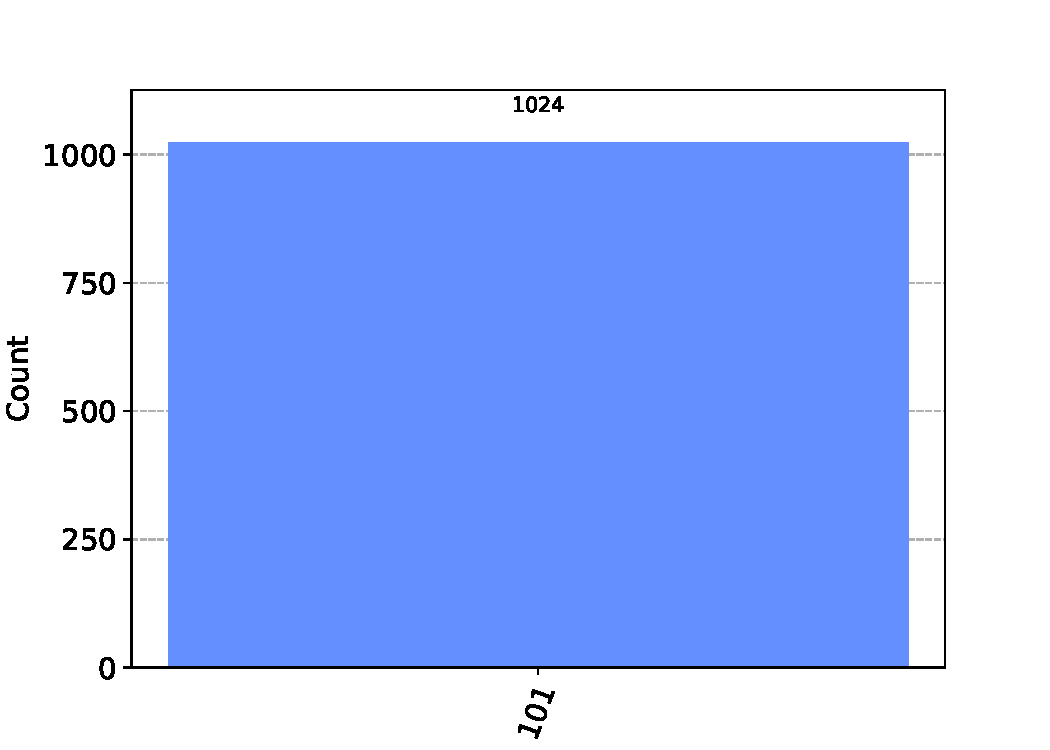
\includegraphics[scale=.5]{images/5_Implementation/half_adder_local_result.pdf}
    \caption{The result of executing the Quantum Half Adder circuit using the Aer Simulator}
\end{figure}

We can note that the result of the output $101=\ket{101}=\ket{AB'O'}=\ket{ASC_{out}}$. To read
the output with the correct endianness we must invert it and we shall read it as $\ket{C_{out}SA}$.
If we exclude qubit $A$ the result is $10_2$ which is $2$ in decimal.

Running the circuit with the same initial states for $A,B$ and $O$ the IBM Osaka Quantum Computer
gives the following result show in Figure (5.5).

\begin{figure}[!ht]
    \centering
    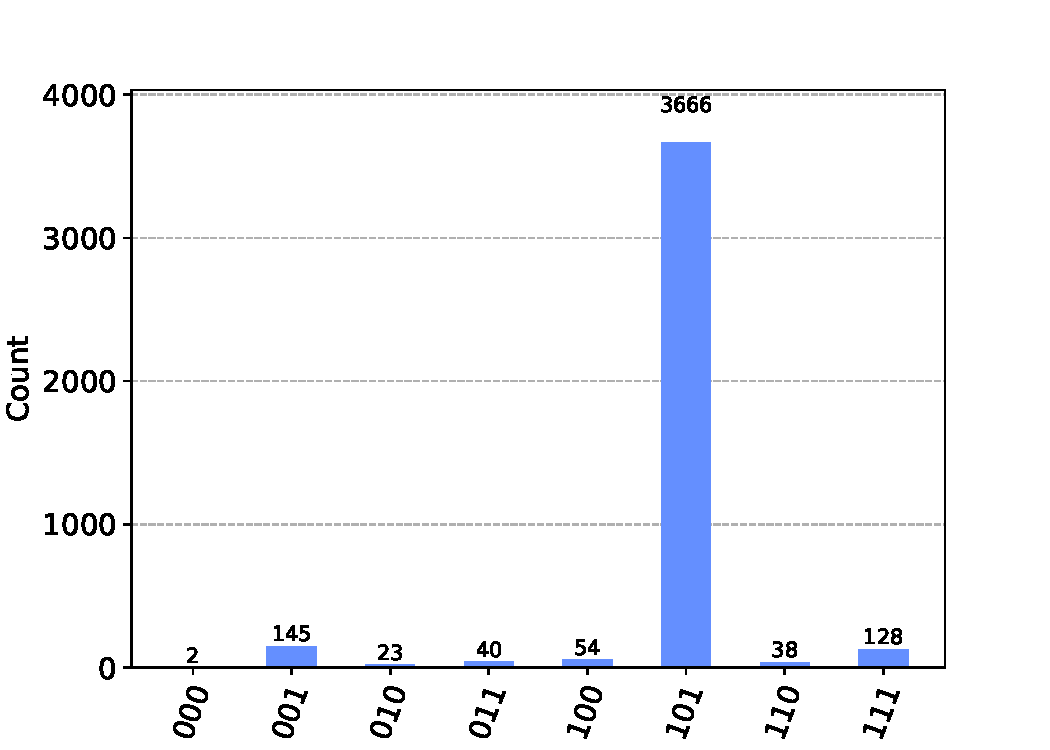
\includegraphics[scale=.5]{images/5_Implementation/half_adder_ibmq_result.pdf}
    \caption{The result of executing the Quantum Half Adder circuit on the IBM Osaka Quantum Computer}
\end{figure}

We can clearly see that the Quantum Computer resulted in more outputs that the simulator. This is due
to errors while executing the circuit for 4096 times. Although some times the Quantum Computer gave
the wrong answers, the most probable output was the correct one ($101$), with a probability of
$\sim 89.5\%$.
\newpage
\section{The Quantum Full Adder}

In this section we are going to construct, using the Qiskit SDK, a quantum circuit that implements the classic Full-Adder circuit.
We are also going to extend this circuit to compute the full addition of any $n$-qubit inputs.

\subsection{Analysing the diagram and logic of the Quantum Full-Adder}

\begin{figure}[ht]
    \centering
    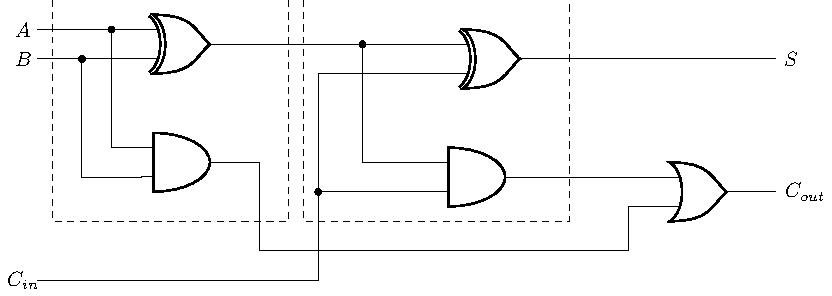
\includegraphics{images/5_Implementation/classical_fulladder_diagram.pdf}
    \caption{The classical Full-Adder circuit diagram}
\end{figure}

The Full-Adder circuit is a circuit that computes the sum $S$ and carry $C_{out}$ of two 1-bit inputs $A$ and $B$ whilist regarding a possible 1-bit
carry from some previous addition $C_{in}$. This is a much more complex circuit than the previously mentioned Half-Adder. It requires two XOR gates,
two AND gate and on OR gate. Although it seems that this circuit is bigger it can be made more simple by just considering two groups of gates. We
have indicated with two dash-lined boxes the gate-groups that are equivalent to Half-Adder circuits.

The first Half-Adder takes inputs $A$ and $B$ and produces two outputs $S_1$ and $C_1$. The second Half-Adder takes inputs $S_1$ and $C_{in}$ and produces
$S$ (which is the sum of $A + B + C_{in}$) and $C_2$. At last an OR gate is applied to $C_1$ and $C_2$ producing $C_{out}$, the carry out.

\begin{table}[ht]
    \centering
    \begin{tabular}{ccc|cc}
        $A$ & $B$ & $C_{in}$ & $S = A \oplus B \oplus C_{in}$ & $C_{out} = (A \oplus B)\cdot C_{in} + A \cdot B$ \\
        \hline
        $0$ & $0$ & $0$ & $0$ & $0$ \\
        $0$ & $1$ & $0$ & $1$ & $0$ \\
        $1$ & $0$ & $0$ & $1$ & $0$ \\
        $1$ & $1$ & $0$ & $0$ & $1$ \\
        $0$ & $0$ & $1$ & $1$ & $0$ \\
        $0$ & $1$ & $1$ & $0$ & $1$ \\
        $1$ & $0$ & $1$ & $0$ & $1$ \\
        $1$ & $1$ & $1$ & $1$ & $1$ \\
    \end{tabular}
    \caption{The truth table of the classical Full-Adder circuit}
\end{table}

We are going to implement the quantum-equivalent with the same techinque that we used to make the quantum Half-Adder circuit.
Just like the quantum Half-Adder, the AND gates need additional \say{garbage} qubits to be implemented in a quantum fashion.
Let $\ket{O}$ be the \say{garbage} qubit that will help to simulate the AND function. Also, let $\ket{A}$, $\ket{B}$ and $\ket{C_{in}}$
be the inputs.

\begin{figure}[ht]
    \centering
    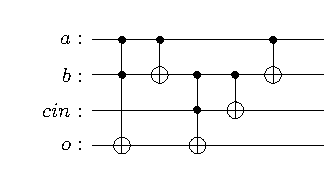
\includegraphics{images/5_Implementation/full_adder.pdf}
    \caption{The diagram of the quantum Full-Adder with slices that indicate each computational step}
\end{figure}

We are going to enumerate through all of the computational steps:
\begin{enumerate}
    \item $\ket{O} = CCNOT\ket{A,B,O} = \ket{C_1}$
    \item $\ket{B} = CNOT\ket{A,B} = \ket{S_1}$
    \item $\ket{C_1} = CCNOT\ket{S_1,C_{in},C_1} = \ket{C_{out}}$
    \item $\ket{S_1} = CNOT\ket{S_1,C_{in}} = \ket{S}$
    \item $\ket{B'} = CNOT\ket{A,S_1} = \ket{B}$
\end{enumerate}

We can see that steps 1-2 and 3-4 are gate sequences matching the behaviour of the quantum Half-Adder circuit. This means that we can replace
those gates with a gate that implements the quantum Half-Adder. Let $QHA$ be a unitary operator:

\begin{equation}
    \centering
    QHA = \begin{bmatrix}
        1 & 0 & 0 & 0 & 0 & 0 & 0 & 0  \\
         0 & 0 & 0 & 0 & 0 & 0 & 0 & 1  \\
         0 & 0 & 1 & 0 & 0 & 0 & 0 & 0  \\
         0 & 1 & 0 & 0 & 0 & 0 & 0 & 0  \\
         0 & 0 & 0 & 0 & 1 & 0 & 0 & 0  \\
         0 & 0 & 0 & 1 & 0 & 0 & 0 & 0  \\
         0 & 0 & 0 & 0 & 0 & 0 & 1 & 0  \\
         0 & 0 & 0 & 0 & 0 & 1 & 0 & 0  \\
         \end{bmatrix}
\end{equation}

Now we can edit Figure 5.5 by using the $QHA$.

\begin{figure}[ht]
    \centering
    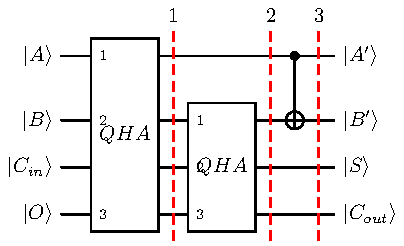
\includegraphics{images/5_Implementation/combinational_full_adder.pdf}
    \caption{The combinational quantum Full-Adder made with two Quantum Half-Adders}
\end{figure}

\subsection{The Python3 implementation}

Just like the Half-Adder implementation, we need to import the two basic classes: \\\mintinline{python3}|QuantumCircuit| and
\mintinline{python3}|QuantumRegister|. We initialize the \mintinline{python3}|circuit| object with the appropriate 1-qubit
registers $A,B,C_{in}$ and $O$.

\begin{listing}[ht]
    \begin{minted}{python3}
        from qiskit import QuantumCircuit, QuantumRegister

        a = QuantumRegister(1, name="A")
        b = QuantumRegister(1, name="B")
        cin = QuantumRegister(1, name="Cin")
        o = QuantumRegister(1, name="O")
        circuit = QuantumCircuit(a, b, cin, o)
    \end{minted}
    \caption{Initializing the quantum Full-Adder circuit}
\end{listing}

According to Figure 5.5 we have to apply five computational steps.

\begin{listing}[ht]
    \begin{minted}{python3}
        circuit.ccx(a, b, o)
        circuit.cx(a, b)
        circuit.ccx(b, cin, o)
        circuit.cx(b, cin)
        circuit.cx(a, b)
    \end{minted}
    \caption{The computations that implement the quantum Full-Adder}
\end{listing}

We can also create a custom gate to implement the Full-Adder using Half-Adders. This can be achieved my re-implementing the
quantum Half-Adder as shown in 5.1.3. and creating a new gate out of that circuit by using the \mintinline{python3}|circuit.to_gate()|
method.

\begin{listing}[ht]
    \begin{minted}{python3}
        from qiskit import QuantumCircuit, QuantumRegister
        # re-implement the half-adder circuit
        half_adder = QuantumCircuit(3)
        half_adder.ccx(0, 1, 2)
        half_adder.ccx(1, 2)
        half_adder_gate = half_adder.to_gate() # create the new gate
    \end{minted}
    \caption{Creating the Half-Adder gate}
\end{listing}

Then we can append the gate to the Full-Adder circuit by the \mintinline{python3}|circuit.append()| method. This method takes
a quantum gate as the first parameter and a list of quantum registers for the second parameter.

\begin{listing}[ht]
    \begin{minted}{python3}
        circuit.append(half_adder_gate, (a[:] + b[:] + cin[:]))
        circuit.append(half_adder_gate, (b[:] + cin[:] + o[:]))
        circuit.cx(a, b) # don't forget to restore b
    \end{minted}
    \caption{Implementating the Full-Adder with the Half-Adder gate}
\end{listing}

It is evident that Listings 5 and 7 are equivalent, they produce the exact same output. Listing 7 has the advantage of being
of a much more modular design which helps with code maintanabilty. Although it is out of the scope of this thesis we wanted
to point this design choice for the sake of transparency.

In the same spirit we can create a custom gate for the Full-Adder. Let $QFA$ be a unitary operator:

\begin{equation}
    QFA = \begin{bmatrix}
        1 & 0 & 0 & 0 & \cdots & 0 & 0 & 0  \\
         0 & 0 & 0 & 0 & \cdots & 1 & 0 & 0  \\
         0 & 0 & 0 & 0 & \cdots & 0 & 1 & 0  \\
         0 & 0 & 0 & 0 & \cdots & 0 & 0 & 0  \\
         \vdots & \vdots & \vdots & \vdots & \ddots & \vdots & \vdots & \vdots \\
         0 & 0 & 0 & 0 & \cdots & 0 & 0 & 0  \\
         0 & 0 & 0 & 0 & \cdots & 0 & 0 & 0  \\
         0 & 0 & 0 & 0 & \cdots & 0 & 0 & 0  \\
         \end{bmatrix}
\end{equation}

\begin{listing}[ht]
    \centering
    \begin{minted}{python3}
        from qiskit import QuantumCircuit, QuantumRegister
    
        a = QuantumRegister(1, name="a")
        b = QuantumRegister(1, name="b")
        cin = QuantumRegister(1, name="cin")
        o = QuantumRegister(1, name="o")
        circuit = QuantumCircuit(a, b, cin, o)

        circuit.ccx(a, b, o)
        circuit.cx(a, b)
        circuit.ccx(b, cin, o)
        circuit.cx(b, cin)
        circuit.cx(a, b)
        full_adder_gate = circuit.to_gate()
    \end{minted}
    \caption{Creating the Full-Adder gate}
\end{listing}
\newpage

We can now use the Full-Adder gate to implement much bigger quantum circuits without too much trouble. We want to point out that
this design is not particulary efficient as it uses one \say{garbage} qubit \cite{Feynman1984}. For the sake of simplicity
we are going to use this circuit as it is very straight-forward to understand.

\subsection{Extending the circuit to $n$-qubits}

The Full-Adder circuit in subsection 5.2.2 is not very useful as it can only compute the sum of 1-qubit registers. In this section
we are going to use all of the previous knowledge to create a Full-Adder circuit that can compute the sum of $n$-qubit register inputs.

By using the gate that we devised in Listing 8, we can create the Quantum Ripple Carry Adder.

For each $n$-qubits iterate over the quantum registers and apply the $QFA$ gate. We have to note that at then end of each iteration
the circuit must apply a SWAP gate on qubit $Cin_{i+1}$ and $C_{out}$. This must be applied at the end of each iteration because
$C_{out}$ stores the carry-out from the $QFA$ and it must be carried down to the next carry-in qubit for the next iteration. This
SWAP gate must not be applied at the end of the circuit because it will swap the last sum $S_{n-1}$ qubit and the $Overflow$ qubit.

\begin{listing}[ht]
    \centering
    \begin{minted}{python3}
        from qiskit import QuantumCircuit, QuantumRegister

        n = -1 # init n to a negative integer
        while n < 0:
            n = input("Input an integer (>0): ")

        a = QuantumRegister(n, name="A")
        b = QuantumRegister(n, name="B")
        cin = QuantumRegister(n, name="Cin")
        o = QuantumRegister(1, name="Cout")
        circuit = QuantumCircuit(a, b, cin, o)

        # create the full adder gate
        full_adder = QuantumCircuit(4)
        full_adder.ccx(0, 1, 3)
        full_adder.cx(0, 1)
        full_adder.ccx(1, 2, 3)
        full_adder.cx(1, 2)
        full_adder.cx(0, 1)
        full_adder_gate = full_adder.to_gate()

        # append the gate to complete the circuit logic
        for i in range(n):
            circuit.append(full_adder_gate,  (a[i], b[i], cin[i], o[:]))
            if i+1 < n:
                circuit.swap(cin[i+1], o)
    \end{minted}
    \caption{Creating the Quantum Ripple Carry Adder}
\end{listing}

\begin{figure}[!ht]
    \centering
    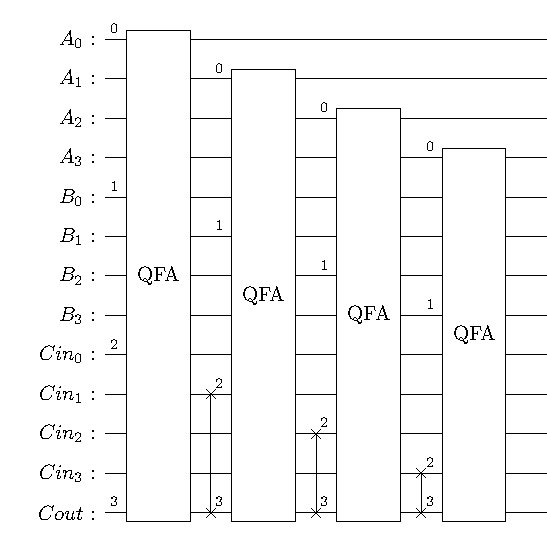
\includegraphics[height=6.5cm]{images/5_Implementation/quantum_ripple_carry_adder.pdf}
    \caption{The circuit diagram of a Quantum Ripple Carry Adder with $n=4$}
\end{figure}

\section{The Quantum Adder-Subtractor}

In this section we are going to construct using the Qiskit SDK the quantum cirucit of the Adder-Subtractor. This will
be the final version of the integer addition-subtraction unit of the Quantum Arithmetic Logic Unit.

\subsection{Analysing the diagram and logic of the Adder-Subtractor circuit}

The Adder-Subtractor circuit, is a digital circuit that computes the sum or the difference of two $n$-bit inputs
and produces an $n$-bit sum or difference, denoted by $O$, and an carry-out overflow bit $C_{overflow}$. This
digital circuit is constructed using the Ripple Carry Adder circuit. As mentioned in Chapter 2, binary subtraction
can be implemented by addition if we take the 2s-complement of the subtrahend and sum it with the minuend. This
saves us from using two different circuits - it takes less logic gates to implement the two operations.

\begin{figure}[!ht]
    \centering
    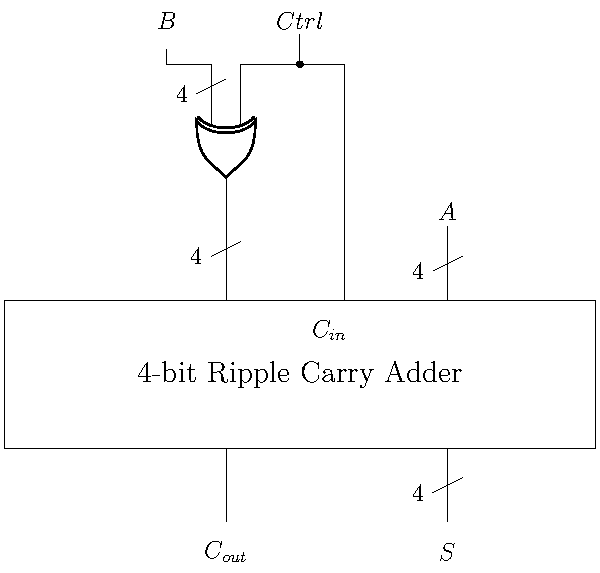
\includegraphics[height=6cm]{images/5_Implementation/classical_adder_subtractor.pdf}
    \caption{The diagram of the classical Adder-Subtractor circuit}
\end{figure}

The Adder-Subtractor works by having one extra wire, denoted as $CTRL$ in the diagram, that controls the mode
of the circuit: zero for addition and one for subtraction. We will skip the first mode because we have covered
that in the previous subsection. The more interesting part is the subtraction mode.

While in subtraction mode, input $B$ and $CTRL$ bit are XOR'ed together to produce the 1s-complement of $B \rightarrow B'$.
To get the 2s-complement, we need to add one to $B' + 1$. This can be done by supplying the $C_{in}$ input of the
4-bit Ripple Carry Adder with the $Ctrl$ wire.

To implement this quantum circuit we are going to need the $QRCA$ gate that we created on the previous subsection and
$n+1$ CNOT gates, so that we can take the 1s-complement of input $B$ and $C_{in_{0}}$. First we apply the CNOT gate, with
the control qubit set to $Ctrl$ and target each qubit of register $B$. We also do the same for the $C_{in_{0}}$ qubit.
Finally we apply the $QRCA$ - the quantum Ripple Carry Adder. This will transform register $C_{in}$ into the register $Out$
which essential stores either the summation or difference of input quantum registers $A$ and $B$.

\subsection{The Python3 implementation}

For this implementation we are going to use the Quantum Ripple Carry Adder, discussed in the previous section.
First, we are going to initialize all the apropriate registers, $A$ and $B$ which store the terms, $CTRL$ which
stores information about the mode of the unit, $C_{in}$ which is either initialized to all-zeros ($\ket{0^{\otimes n}}$)
or all-zeros except the LSB (least significant (qu)bit) which is set by $CTRL$.

\begin{listing}[!ht]
    \centering
    \begin{minted}{python3}
        from qiskit import QuantumCircuit, QuantumRegister

        ctrl = QuantumRegister(1, name="Ctrl")
        a = QuantumRegister(n, name="A")
        b = QuantumRegister(n, name="B")
        cin = QuantumRegister(n, name="Cin")
        cout = QuantumRegister(1, name="Cout")
        circuit = QuantumCircuit(ctrl, a, b, cin, o)
    \end{minted}
    \caption{Initialization of the Adder-Subtractor circuit}
\end{listing}

Next we are going to invert all qubits of register $B$ by applying the CNOT gate to each qubit controlled by 1-qubit
register $CTRL$. We also invert the LSB of register $C_{in}$ to acquire the 2s-complement of register $B$. After that,
we apply the QRCA gate and finally un-compute reigster $B$.

\begin{listing}[!ht]
    \centering
    \begin{minted}{python3}
        for i in range(n):
            circuit.cx(ctrl, b[i])
        circuit.cx(ctrl, cin[0])
        circuit.append(rca, (a[:] + b[:] + cin[:] + o[:]))
        for i in reversed(range(n)):
            circuit.cx(ctrl, b[i])
    \end{minted}
    \caption{Step-by-step instructions of the quantum Adder-Subtractor circuit}
\end{listing}

\begin{figure}[!ht]
    \centering
    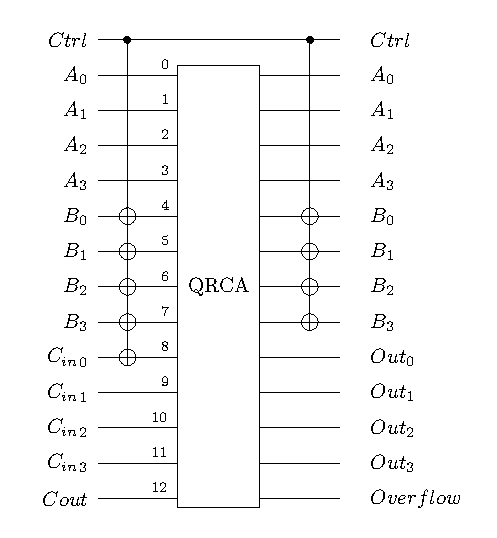
\includegraphics{images/5_Implementation/quantum_adder_subtractor.pdf}
    \caption{The diagram of the quantum Adder-Subtractor circuit}
\end{figure}
\newpage
\section{The Quantum Integer Multiplier}

In this section we are going to implement a quantum circuit that computes the product
of two 2-qubit numbers. We are going to first discuss the design of the classic circuit
and then focus on the implementation of its quantum analogue using the Qiskit SDK.

\subsection{Analysing the diagram and logic of the classical Integer Multiplier circuit}

The Integer Multiplier circuit, or just the Multiplier circuit, is a digital circuit that
takes two $n$-bit inputs and computes their arithmetic product. The circuit we are going to
analyse implements the binary multiplication algorithm, by first computing the partial products
and then summing them up to produce the final product \cite{ManoCiletti2018}.

Let $A$ and $B$ be two $n$-bit classic registers. For the purposes of simplicity let $n = 2$.
To compute their multiplication product we first produce the \textit{partial products} of $A \times B$.
This is done digitally by applying an AND gate on every $A_i$ and $B_j$ pair. Then we apply a Half-Adder
for the partial products. We note that the LSB of $PP$ does not need to be added to the Half-Adders.

\begin{table}[ht]
    \centering
    \begin{tabular}{ccccc}
        $$ & $$ & $$ & $B_1$ & $B_0$ \\
        $$ & $$ & $+$ & $A_1$ & $A_0$ \\
        $$ & \cline{2-4}
        $$ & $$ & $$ & $PP_1$ & $PP_0$ \\
        $$ & $\times$ & $PP_3$ & $PP_2$ & $$ \\
        \hline
        $$ & $P_3$ & $P_2$ & $P_1$ & $P_0$ \\
    \end{tabular}
    \caption{Multiplication for two 2-bit integers}
\end{table}

\begin{figure}[ht]
    \centering
    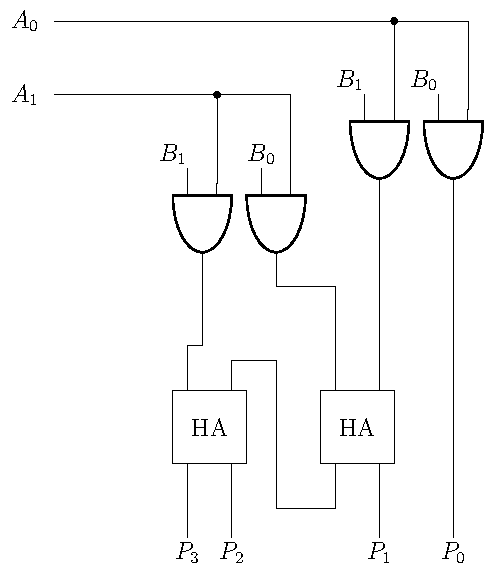
\includegraphics[height=6cm]{images/5_Implementation/classical_2bit_multiplier.pdf}
    \caption{The diagram of the classical Multiplier circuit for two 2-bit inputs}
\end{figure}

\subsection{Implementing the Quantum Multiplier in Python}

The quantum implementation is an expensive circuit, qubit-wise, as it needs to compute the
partial products. As we mentioned previously, the AND function can be simulated by the Toffoli gate
by using one \say{garbage} qubit to store the conjunction of the two conrtol qubits, thus we
need $n^2$ qubits to store the partial products of two $n$-qubit inputs.

As always we initialize the circuit with the two 2-qubit input registers $A$ and $B$. We also
include in our circuit the $2n^2$-qubit output quantum register.

\begin{listing}[ht]
    \centering
    \begin{minted}{python3}
        from qiskit import QuantumCircuit, QuantumRegister

        n = 2
        a = QuantumRegister(n, name="A")
        b = QuantumRegister(n, name="B")
        out = QuantumRegister(2*n**2, name="out")

        circuit = QuantumCircuit(a, b, out)
    \end{minted}
    \caption{Initialization of the quantum Multiplier circuit}
\end{listing}

We proceed to compute the partial-products of $A \times B$ by applying the CNOT gate for each
qubit-pair $A_iB_j$.

\begin{listing}[ht]
    \centering
    \begin{minted}{python3}
        k = 0
        for i in range(n):
            for j in range(n):
                circuit.cx(a[i], b[j], out[k])
                k += 1
    \end{minted}
    \caption{Computing the partial-products for the quantum Multiplier circuit}
\end{listing}

Despite the expensive nature of the circuit, the overall compexity is pretty low due to the modular
nature of the circuit. We can use the $QFA$ from Section 5.2 to implement the additions of the partial products
but we have to be careful as to which pair of inputs we supply the $QFA$s.

\begin{listing}[ht]
    \centering
    \begin{minted}{python3}
        circuit.append(qfa, (out[1], out[2], out[4], out[5]))
        circuit.append(qfa, (out[3], out[5], out[6], out[7]))
    \end{minted}
    \caption{Summing the partial-products to compute the product of $A\times B$}
\end{listing}

To produce the products we need to compute the sum of $P_1+P_2$. This in-turn will produce a sum and a carry-out,
$P_1$ and $C_{out_0}$. The $C_{out_0}$ will be used for the next addition with $P_3$. Finally, after the last
addition we have computed the product of $A \times B$. The output is stored in qubits $Out_0$, $Out_4$, $Out_6$ and
$Out_7$, with $Out_7$ be the most-significant qubit of the product.

\begin{figure}[ht]
    \centering
    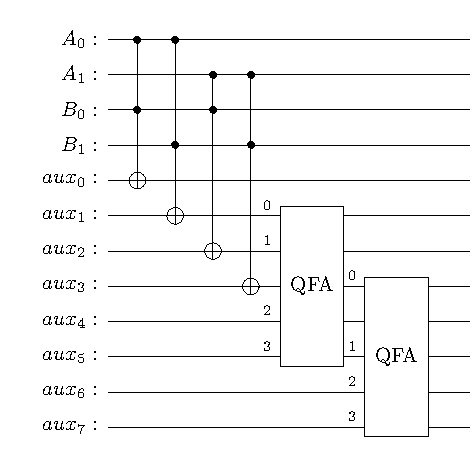
\includegraphics{images/5_Implementation/quantum_2bit_multiplier_with_qfa.pdf}
    \caption{The complete quantum Multiplier unit for 2-qubit inputs}
\end{figure}
\section{The Quantum Integer Comparator}

In this section we are going to analyse a classical circuit that compares two integer numbers
$A$ and $B$ and produces three different signals:

\begin{enumerate}
    \item signal when $A$ is equal with $B$
    \item signal when $A$ is greater than $B$ and
    \item signal when $A$ is less than $B$
\end{enumerate}

\subsection{Analysing the diagram and logic of the classical Comparator circuit}

In the digital logic, a comparator circuit is used to compare two binary encoded numbers. The encoding of (signed or unsigned)
is particularly useful because in the case of the signed-magnitude encoding, we just need to compare the most-significant bits
of the two numbers. If the numbers have different signs then we need only to check their signs, that means their most-significant
bits, and in the later case, when they have the same sign, we need to check their absolute magnitude \cite{Giannakopoulos2015}.

For the purposes of simplicity, we are going to analyze a \textit{serial binary comparator} circuit.

Some classical computers have the capabilities to compute multiple comparison logics like: $>$, $<$, $\ge$, $\le$, $=$ and $\neq$.
Some other computers can only produce a sset of the those comparisons. We are going to analyze only a sset of those comparisons,
specificaly we are going to analyze and construct a digital logic circuit that computes only $=$, $\neq$, $<$ and $>$.
We can produce the truth table of a circuit that computes the equality of two 1-bit numbers easily.

\begin{table}[ht]
    \centering
    \begin{tabular}{cc|c}
        $A$ & $B$ & Equals \\
        \hline
        $0$ & $0$ & $=(1)$ \\
        $0$ & $1$ & $\neq(0)$ \\
        $1$ & $0$ & $\neq(0)$ \\
        $1$ & $1$ & $=(1)$ \\
    \end{tabular}
    \caption{The truth table of a circuit that implements equality check between two bits}
\end{table}

Note that the truth table is equivelant to the XNOR gate's truth table. In fact, if we had $n$-bit inputs, we would just need
$n$ XNOR gates and a $n$-input AND gate to implement a $n$-input equality comparator.

Next, we can implement a circuit that compares two bits and produces $0\text{ when }<$ and $1\text{ when }\geq$

\begin{table}[ht]
    \centering
    \begin{tabular}{cc|c}
        $A$ & $B$ & Greater Equals or Less than \\
        \hline
        $0$ & $0$ & $1(\geq)$ \\
        $0$ & $1$ & $0(<)$ \\
        $1$ & $0$ & $1(\geq)$ \\
        $1$ & $1$ & $1(\geq)$ \\
    \end{tabular}
    \caption{The truth table of a circuit that implements the "greater or equals than" between two bits}
\end{table}

The boolean expression that implements this circuit is the following:

\begin{equation}
    F = A + B'
\end{equation}
Putting it all together we construct the following logic circuit.

\begin{figure}[ht]
    \centering
    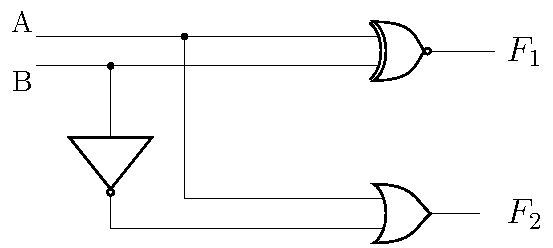
\includegraphics[height=4cm]{images/5_Implementation/classical_1bit_comparator.pdf}
\end{figure}

\begin{equation}
    \text{Where }F_1 =
    \begin{cases}
        A = B, \text{ when }1 \\
        A \neq B, \text { when }0
    \end{cases}
    \text{ and where }
    F_2 =
    \begin{cases}
        A \geq B, \text{ when }1 \\
        A < B, \text{ when }0
    \end{cases}
\end{equation}

\begin{table}[ht]
    \centering
    \begin{tabular}{cc|cc}
        $A$ & $B$ & $F_1$ & $F_2$ \\
        \hline
        $0$ & $0$ & $1$ & $1$ \\
        $0$ & $1$ & $0$ & $0$ \\
        $1$ & $0$ & $0$ & $1$ \\
        $1$ & $1$ & $1$ & $1$ \\
    \end{tabular}
    \caption{The truth table of the classical comparator circuit for two bits}
\end{table}
\newpage
We are going to present the diagram for a quantum comparator of integers. The design is based on the work of Nascimento,
Kowanda and de Oliveira \cite{NKO2006}. The design specifies two important constructs:

\begin{enumerate}
    \item the unitary gate $S$ - a quantum gate that computes the difference of two-qubits
    \item the inverse of the unitary gate $S$, $S^\dag$ - a quantum gate that un-computes the computed difference
\end{enumerate}

We use the $S^\dag$ gate to restore $B$ to its initial state, because $S$ gate computes the difference of $A$ and $B$
and stores it to $B$. Just like the quantum Half-Adder from section 5.1, we un-compute the changes to a particular
qubit so it can be used for some later computation.

\begin{figure}[ht]
    \centering
    \begin{subfigure}{0.3\textwidth}
        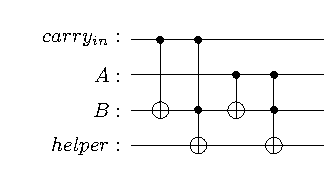
\includegraphics{images/5_Implementation/quantum_nko_sgate.pdf}
        \caption{}
    \end{subfigure}
    \hspace{2.5cm}
    \begin{subfigure}{0.3\textwidth}
        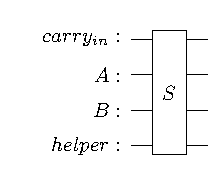
\includegraphics{images/5_Implementation/quantum_nko_sgate_final.pdf}
        \caption{}
    \end{subfigure}
    \begin{subfigure}{0.3\textwidth}
        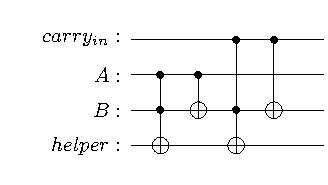
\includegraphics{images/5_Implementation/quantum_nko_sdaggate.pdf}
        \caption{}
    \end{subfigure}
    \hspace{2.5cm}
    \begin{subfigure}{0.3\textwidth}
        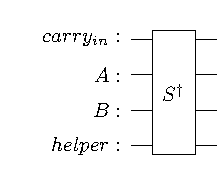
\includegraphics{images/5_Implementation/quantum_nko_sdaggate_final.pdf}
        \caption{}
    \end{subfigure}
    \caption{The unitary $S$ and $S^\dag$ gates' circuit (a, c) and gate (b, d) diagrams}
\end{figure}

To compare two variable-sized quantum registers $A, B$, we need to apply the $S$ gate to 
each pair $A_i,B_i$ and $ancilla_i,ancilla_{i+1}$. Note that we need $n+1$ ancilla qubits
to implement this design. We iteratively apply the above.

Apply a multi-inverse-control CNOT gate to circuit. Control qubits are register $B$'s qubits,
which stores the difference of $A-B$ in 2s-complement, and target the $O_0$ qubit which is the
least-significant qubit of a special purpose register we shall call the \textit{status register}.

Lastly, we copy, by applying a regular CNOT gate, the most-significant qubit of register $B$,
which stores the sign of the difference, to qubit $O_1$ of the status register.

Finally, we uncompute iteratively using the $S^\dag$ gate.

\begin{figure}[ht]
    \centering
    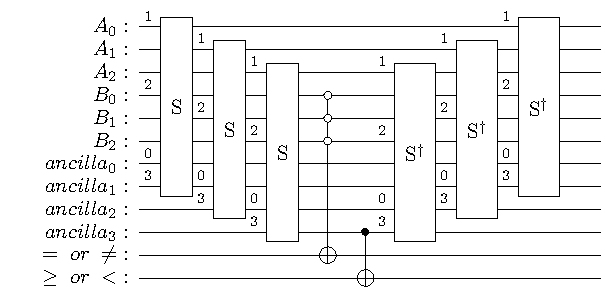
\includegraphics{images/5_Implementation/nko_comparator.pdf}
    \caption{The diagram of the quantum Integer Comparator circuit}
\end{figure}

\subsection{The Python3 Implementation}

To implement the comparator circuit we need to construct the $S$ and $S^\dag$ gates.

\begin{listing}[ht]
    \centering
    \begin{minted}{python3}
        s = QuantumCircuit(4, name="S")
        s.cx(0, 2)
        s.ccx(0, 2, 3)
        s.cx(1, 2)
        s.ccx(1, 2, 3)
        s = s.to_gate()

        sdag = QuantumCircuit(4, name="S_dag")
        sdag.ccx(1, 2, 3)
        sdag.cx(1, 2)
        sdag.ccx(0, 2, 3)
        sdag.cx(0, 2)
        sdag = sdag.to_gate()
    \end{minted}
    \caption{}
\end{listing}

After that we init the main circuit. The size of the registers are fixed to $n=3$, although it can
be set to any positive integer. We also include some ancilla qubits.

\begin{listing}[ht]
    \centering
    \begin{minted}{python3}
        n = 3
        a = QuantumRegister(n, name="A")
        b = QuantumRegister(n, name="B")
        anc = QuantumRegister(n+1, name="ancilla")
        eq = QuantumRegister(1, name="Eq")
        geq = QuantumRegister(1, name="Geq")

        circuit = QuantumCircuit(a, b, anc, eq, gl, name="NKOComparator")
    \end{minted}
    \caption{}
\end{listing}

\newpage

Following the initialization is the main circuit logic. First apply the $S$ gate to compute
the difference of $A-B$ and store it to $B$.

\begin{listing}[ht]
    \centering
    \begin{minted}{python3}
        # compute diff
        for i in range(n):
            circuit.append(s, (anc[i], a[i], b[i], anc[i+1]))
    \end{minted}
    \caption{}
\end{listing}

After we computed the difference, check if all the qubits of register $B$ are zero.
This can be done by using a Multi-Controlled CNOT Gate (MCX) from the \mintinline{python3}|qiskit.circuit.library|.
We set the MCX gate to use inverted logic for the control qubits, so if every control qubit is in the zero state
the target qubit will be inverted. If every qubit of register $B$ are in the zero state, the two registers stored
the same number thus $A$ and $B$ are equal.

\begin{listing}[ht]
    \centering
    \begin{minted}{python3}
        from qiskit.circuit.library import MCXGate
        circuit.append(MCXGate(n, ctrl_state=0), (b[:] + eq[:]))
    \end{minted}
    \caption{}
\end{listing}

To check if $A$ is greater or less than $B$, we can check the sign qubit of the difference. This is easily
done by applying a CNOT gate to most-significant qubit of the difference.

\begin{listing}[!ht]
    \centering
    \begin{minted}{python3}
        circuit.cx(anc[-1], geq)
    \end{minted}
    \caption{}
\end{listing}

\newpage

Finally, we un-compute by applying the $S^\dag$ gate to the circuit in reverse.

\begin{listing}[ht]
    \centering
    \begin{minted}{python3}
        for i in reversed(range(n)):
            circuit.append(sdag, (anc[i], a[i], b[i], anc[i+1]))
    \end{minted}
    \caption{}
\end{listing}

\begin{listing}[ht]
    \centering
    \begin{minted}{python3}
        from qiskit import QuantumCircuit, QuantumRegister

        n = 3

        a = QuantumRegister(n, name="A")
        b = QuantumRegister(n, name="B")
        anc = QuantumRegister(n+1, name="ancilla")
        eq = QuantumRegister(1, name="eq")
        gl = QuantumRegister(1, name="geq")

        circuit = QuantumCircuit(a, b, anc, eq, geq, name="NKOComparator")

        s = QuantumCircuit(4, name="S")
        s.cx(0, 2)
        s.ccx(0, 2, 3)
        s.cx(1, 2)
        s.ccx(1, 2, 3)
        s = s.to_gate()
            
        sdag = QuantumCircuit(4, name="S_dag")
        sdag.ccx(1, 2, 3)
        sdag.cx(1, 2)
        sdag.ccx(0, 2, 3)
        sdag.cx(0, 2)
        sdag = sdag.to_gate()

        # compute diff
        for i in range(n):
            circuit.append(s, (anc[i], a[i], b[i], anc[i+1]))

        from qiskit.circuit.library import MCXGate
        circuit.append(MCXGate(n, ctrl_state=0), (b[:] + eq[:])) # compute equals
        circuit.cx(anc[-1], geq) # if msb < 0 then a < b else b >= a

        # un-compute diff
        for i in reversed(range(n)):
            circuit.append(sdag, (anc[i], a[i], b[i], anc[i+1]))
    \end{minted}
\end{listing}